\documentclass[12pt]{article}

\usepackage[utf8]{inputenc}
\usepackage{geometry}
\usepackage{amsmath}
\usepackage{amsfonts}
\usepackage{last page}
\usepackage{fancyhdr}
\usepackage{enumitem}
\usepackage{tikz}
\usepackage{xcolor}
\usepackage{sectsty}
\usepackage{caption}
\usepackage{graphicx}
\usepackage{float}

\definecolor{BackgroundColor}{HTML}{ffffff}
\definecolor{FontColor}{HTML}{152525}
\definecolor{SectionColor}{HTML}{216666}
\definecolor{SubSectionColor}{HTML}{3b8787}
\definecolor{SubSubSectionColor}{HTML}{4aa8a8}

\definecolor{GreenNC}{HTML}{2ED390}
\definecolor{BlueNC}{HTML}{c7f2f8}
\definecolor{DarkBlueNC}{HTML}{4aa8a8}

\newcommand\nodegui{NetworkOperatorGUI}
\newcommand\nodeui{IUserInterface}
\newcommand\nodepm{PluginManager}
\newcommand\nodeconf{Configurator}
\newcommand\nodeo{NetworkOperator}
\newcommand\nodeoc{ActionRequestCreator}
\newcommand\nodeop{ActionRequestProcessor}
\newcommand\nodeci{ICommunicationInterface}
\newcommand\nodeos{OperandSelector}
\newcommand\nodenm{NetworkCommunicator}
\newcommand\nodeml{MouseShrARC}
\newcommand\nodekl{KeyboardShrARC}
\newcommand\nodems{MouseShrARP}
\newcommand\nodeks{KeyboardShrARP}
\newcommand\nodeses{ScreenEdgeSelector}

\renewcommand{\contentsname}{Obsah}
\renewcommand{\figurename}{Obr.}
\makeatletter
\renewcommand{\@seccntformat}[1]{}%disables printing results of section numbering system at the beginning of headline of numbered parts of the article
\renewcommand\paragraph{%
    \@startsection{paragraph}{4}{0mm}%
       {-\baselineskip}%
       {.5\baselineskip}%
       {\normalfont\normalsize\bfseries}}
\makeatother

\pagecolor{BackgroundColor}
\color{FontColor}
\sectionfont{\color{SectionColor}}
\subsectionfont{\color{SubSectionColor}}
\subsubsectionfont{\color{SubSubSectionColor}}

\tikzstyle{mynodestyle} = [rectangle, minimum size=20pt, text=FontColor]
\tikzstyle{bn} = [mynodestyle, draw=BlueNC, fill=BlueNC]
\tikzstyle{gn} = [mynodestyle, draw=GreenNC, fill=GreenNC]
\tikzstyle{dn} = [mynodestyle, draw=DarkBlueNC, fill=DarkBlueNC]

\tikzset{>=latex, every picture/.style={line width=1pt}}

\geometry{a4paper, total={190mm, 277mm}, left=20mm, right=20mm, top=20mm, bottom=20mm}
\setlength{\parindent}{0mm}

\title{Dokumentace NetworkOperatoru, zápočtového programu z předmětů NPRG035, NPRG038, NPRG057 a NPRG064}
\date{ZS/LS 2016/2017}
\author{Václav Balcar, 2. ročník, 31. studijní skupina}

\fancyhf{}
\lhead{Dokumentace}
\rhead{NetworkOperator}
\rfoot{\thepage}
\pagestyle{fancy}

\graphicspath{{images/}}

\begin{document}
\pagenumbering{gobble}
\maketitle
\newpage
\pagenumbering{arabic}
\tableofcontents
\newpage
\section{Úvod}
V rámci plnění požadavků specifikace jsem se snažil být maximálně přesný a až na několik interních implementačních detailů a úpravě jedné části GUI za účelem zvýšení uživatelské přívětivosti jsem ji, věřím, dodržel. Není-li tedy (implicitně) uvedeno jinak, funguje daná část programu tak, jak uvádí specifikace (pokud se výjimky z tohoto pravidla přeci jen vyskytnou, nebylo to mým záměrem a u zásadních částí programu by se tak stát nikdy nemělo).
\newpage

\section{Uživatelská dokumentace}

\subsection{Rychlé seznámení se s programem}
NetworkOperator je program vytvořený primárně za účelem jednoduchého provádění operací s počítači připojenými k jedné počítačové síti. Podstata těchto operací není předem nijak definovaná, programátoři implementující konkrétní operace mají v tomto volnou ruku.

\subsection{Nativní funkce programu}
NetworkOperator poskytuje uživateli základní kontrolu nad každou operací - umožňuje operaci spustit nebo pozastavit. Dále zprostředkovává možnost zobrazení přehledu operace a spuštění případného konfigurátoru nějaké operace nebo její součásti. Poslední naivní funkcí programu je automatické spouštění vybraných operací bezprostředně po spuštění programu.

\subsection{Implementované operace}
NetworkOperator sám od sebe neumí provádět žádnou uživateli přístupnou operaci, v odevzdané verzi jsou však dodatečně implementovány dvě operace - Keyboard Sharing a Mouse Sharing.
Operace lze provádět s počítači z jedné broadcast domény, na kterých je spuštěn NetworkOperator.

\subsubsection{Mouse Sharing}
Jak název napovídá, tato operace umožňuje sdílet myš mezi počítači. Pro sdílení myši mezi všemi počítači není třeba dělat nic komplikovaného, stačí jen vzít myš a přesunout kurzor z jednoho počítače na druhý, jako by se jednalo o monitory připojené k jednomu počítači. Všechny myši všech počítačů, které jsou vzájemně propojeny, pak ovládají jeden kurzor. Předpokladem je správně nakonfigurované vzájemné rozmístění počítačů (resp. jejich monitorů), k čemuž je v programu připraven přehledný konfigurátor.

\subsubsection{Keyboard Sharing}
Jedná se o dodatečnou operaci k operaci "Mouse Sharing" umožňující vkládat do ovládaného počítače vstupy klávesnice. Není možné sdílet pouze klávesnici, vždy je nutné sdílet i myš, protože přejížděním myší po monitorech se vybírá ovládaný počítač.

\subsection{Ovládání programu}
Program je ovládán výhradně přes grafické uživatelské rozhraní. Viz část o GUI v programátorské dokumentaci.

\subsection{Požadavky na provoz programu}
NetworkOperator vyžaduje operační systém Windows 2000 nebo vyšší, cca 7MB místa na disku a vhodné síťové rozhraní. Žádné další požadavky kladeny nejsou.

\newpage
\section{Programátorská dokumentace}

\subsection{Základní idea}
NetworkOperator je přenesením obecného matematického operátoru do světa spolupracujících počítačů. Podívejme se například na binární operaci sčítání nad množinou celých čísel, tj. výraz $a+b$ kde $a,b\in \mathbb{Z}$. Na daný výraz je možné pohlížet jako na situaci, kdy "někdo" má požadavek "b" třídy "+" na prvek "a" kompatibilní s požadavkem "b". Výsledkem dané situace je, že prvek "a" přejde v případě splnění všech předpokladů do stavu $a+b$. Také můžeme říct, že "b" je požadavek na akci na prvku "a", který má zpracovat procesor požadavků na akci definovaný operací sčítání. Otázkou zůstává, kde se berou ony požadavky na akci. To je ovšem v zásadě jedno, můžeme říct, že mají svého tvůrce, entitu, která si zvolí nějaký konkrétní operand, kterému předá svůj požadavek na akci. Ve světě matematiky může být tímto tvůrcem například matematik, ve světě počítačů počítačový program. Dále je třeba požadavek na akci ke zvolenému operandu doručit pomocí nějakého konkrétního komunikačního kanálu, se kterým lze pracovat pomocí komunikačního rozhraní. Zde by jako modelový příklad ze světa matematiky mohla posloužit kalkulačka, která má komunikační rozhraní implementované pomocí tlačítek a komunikační kanál, kterým je program, který kalkulačka vykonává.
Když tedy matematik zadá do kalkulačky $1+2$, stává se tvůrcem požadavku na akci "2" operace sčítání na prvek "1". Ve chvíli, kdy nechává kalkulačku výraz vyhodnotit, informuje jedničku o svém požadavku na akci a ta, protože byly splněny všechny předpoklady pro provedení akce, provede požadovanou akci sama na sobě a výsledkem je trojka.
Pro operace s aritou vyšší než 2 je situace analogická.
Přeneseme-li tuto myšlenku do světa navzájem komunikujících počítačů, zjistíme, že zde bez problému funguje. Spolupracují-li spolu počítače $A,B\in S$, kde S je množina počítačů, které spolu mohou komunikovat, může vypadat jejich spolupráce jako posloupnost následujících kroků: Počítač "B" pošle požadavek na akci "b" třídy "o" počítači "A", který, zná-li definici o a existuje-li $a\in A$, provede $a = a o b$.
NetworkOperator je implementací nástroje pro takový typ spolupráce počítačů. Jak přesně je NetworkOperator implementovaný, vysvětlím na schématu architektury NetworkOperatoru.

\subsection{Schéma architektury}
\begin{center}
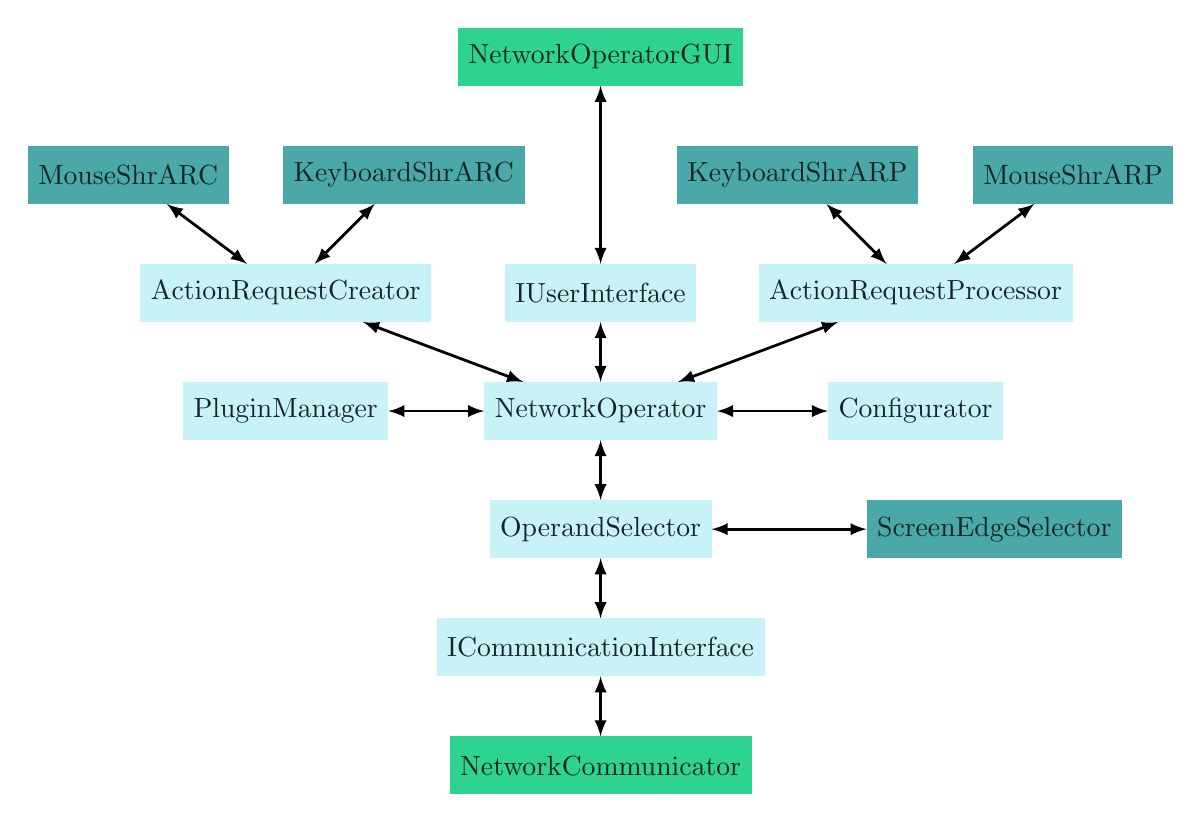
\begin{tikzpicture}
\node[gn] (gui) at (6, 3) {\nodegui};
\node[bn] (ui) at (6, 0) {\nodeui};
\node[bn] (pm) at (2, -1.5) {\nodepm};
\node[bn] (conf) at (10, -1.5) {\nodeconf};
\node[bn] (o) at (6, -1.5) {\nodeo};
\node[bn] (oc) at (2, 0) {\nodeoc};
\node[bn] (op) at (10, 0) {\nodeop};
\node[bn] (os) at (6, -3) {\nodeos};
\node[bn] (ci) at (6, -4.5) {\nodeci};
\node[gn] (nm) at (6, -6) {\nodenm};
\node[dn] (ml) at (0, 1.5) {\nodeml};
\node[dn] (kl) at (3.5, 1.5) {\nodekl};
\node[dn] (ms) at (12, 1.5) {\nodems};
\node[dn] (ks) at (8.5, 1.5) {\nodeks};
\node[dn] (ses) at (11, -3) {\nodeses};
\draw [<->] (gui) -- (ui);
\draw [<->] (ui) -- (o);
\draw [<->] (pm) -- (o);
\draw [<->] (o) -- (conf);
\draw [<->] (oc) -- (o);
\draw [<->] (o) -- (op);
\draw [<->] (kl) -- (oc);
\draw [<->] (ml) -- (oc);
\draw [<->] (op) -- (ks);
\draw [<->] (op) -- (ms);
\draw [<->] (o) -- (os);
\draw [<->] (os) -- (ci);
\draw [<->] (ci) -- (nm);
\draw [<->] (os) -- (ses);
\end{tikzpicture}
\captionof{figure}{Schéma architektury}
\end{center}

\subsection{Implementace základní idee NetworkOperatoru}
NetworkOperator obsahuje několik zásadních součástí: jádro, množinu implementovaných operací a jejich OperandSelectorů, komunikační a uživatelská rozhraní. Mluvíme-li v následujícím textu o složkách, myslíme tím složky v kořenovém adresáři programu.

\subsubsection{Jádro}
To funguje jako načítací program pro většinu ostatních součástí NetworkOperatoru. Také slouží jako propojovací vrstva propojující načtené součástí tím, že poskytuje přístup do svých vnitřních registrů, které jsou naplňovány externími komponentami programu načítanými z příslušných složek v programu. Více o procesu načítání viz podsekce "proces načítání".
Jedinou komponentou, kterou NetworkOperator nenačítá, je uživatelské rozhraní, které musí vytvořit instanci jádra, zaregistrovat se do něj a získat ovladač (controller) jádra. Tento controller umožňuje kromě základních operací jádra, jako je načtení nebo ukončení, zpřístupnit zeregistrované operace. Jádro doplněné operacemi je totiž implementací MVC patternu.
Další významnou funkcí jádra je správa konfiguračních souborů, respektive poskytovaní služby úschovy dat mezi jednotlivými spuštěními programu. Jakákoliv komponenta si může nechat uložit seznam nebo dvourozměrné pole na řetězce převoditelných dat (nebo řetězců jako takových). Tuto funkci, jak název napovídá, zastává Configurator. Každou ukládanou strukturu ukládá do samostatného souboru do složky Configuration.

\paragraph{Proces načítání} je zajištěný třídami PluginManager a Loader, využívá reflection a načítá jednotlivé třídy komponent v následujícím pořadí: OperandSelectory, operace, komunikační rozhraní.

\subsubsection{Operace}
Operací lze NetworkOperatoru dodat libovolné rozumné množství. Pro implementaci operace stačí vytvořit potomka třídy Operation v nějakém dll souboru a tento dll soubor umístit do složky Operations. Každá z nich musí (podle základní idee výše) implementovat ActionRequestCreator, který může v kterýkoliv moment odeslat přes všechna komunikační rozhraní požadavek na akci, ActionRequestProcessor, který zpracovává kompatibilní přijaté požadavky na akci, a obsahovat typ (odpovídající instanci třídy Type) požadovaného OperandSelectoru a název položky, do které požaduje daná operace instanci OperandSelectoru načíst. Tímto způsobem lze snadno dosáhnout nezávistosti OperandSelectorů na konkrétních operacích a také sdílení stejného OperandSelectoru mezi vícero operacemi, čehož se v dodatečně implementovaných operacích využívá.

\subsubsection{OperandSelectory}
Slouží k výběru počítače, kterému bude poslán požadavek na akci. Jeho fungování je de-facto libovolné, každý OperandSelector musí být potomkem třídy OperandSelector a být v dll souboru ve složce OperandSelectors.

\subsubsection{Komunikační rozhraní}
Každé komunikační rozhraní musí implementovat rozhraní ICommunicationInterface a musí být v dll souboru ve složce CommunicationInterfaces. Obecně je NetworkOperator navržený tak, že je možné využívat jakýkoliv způsob komunikace, ovšem ve finální verzi je implementované komunikační rozhraní umožňující komunikaci po počítačové síti. Více o tomto komunikačním rozhraní lze nalézt v sekci "NetworkCommunicator".

\subsection{Iplementované OperandSelectory}
\subsubsection{ScreenEdgeSelector}
Je jediný implementovaný OperandSelector, který funguje tak, že cílový operand se vybírá přejížděním myši po vzájemně sousedních monitorech, přechod funguje stejně jako by se jednalo o více monitorů připojených k jednomu počítači. Sousednost je dána maticí sousednosti, která je definována uživatelskou konfigurací, proto obsahuje konfigurátor (konfigurační okno) umožňující nastavovat vzájemné rozmístění počítačů. Pro uložení matice sousedních operandů interně používá dvourozměrné pole řetězců obsahujících názvy jednotlivých počítačů.

\subsection{Implementované operace}
\subsubsection{Mouse sharing}
Operace umožňující sdílení myši mezi vícero počítači. Uživatelské fungování Mouse sharingu je popsáno v uživatelské dokumentaci. Po technické stránce je operace Mouse sharing zařízena pomocí odchytávání systémových zpráv a jejich následnému přenášení do zvoleného počítače, na němž jsou pomocí Windows API funkcí simulovány. Události související s pohybem kurzoru jsou odchytávány tak, že informace o změně polohy je přenášena nejvýše 60krát za sekundu. Fungování této operace je zajištěno za tímto účelem napsanou knihovnou Mouse.dll, která umožňuje zpracovávat a rušit události myši na úrovni operačního systému pomocí v C\#u napsaných delegátů. Potřebnou transformaci delegátů, případně řízení garbage collectoru, zajišťuje knihovna FunctionMarshaler pracující s .NETími třídami Marshal a GCHandle. Jako OperandSelector používá ScreenEdgeSelector, jako konfuguraci (viz část o GUI) konfiguraci svého OperandSelectoru.

\subsubsection{Keyboard sharing}
Funguje velmi podobnně jako "Mouse sharing", pouze pracuje s klávesnicí a používá knihovnu Keyboard.dll pracující velmi podobně jako knihovna Mouse.dll.

\subsection{NetworkCommunicator}
V této sekci je popsáno, jakým způsobem funguje vzájemné propojení počítačů, které jsou připojeny k jedné počítačové síti (broadcast doméně) a běží na nich NetworkOperator.
NetworkOperator (NetworkOperatorCommunicator.dll) používá ke svému fungování knihovnu ParallelNetworkStream.dll umožňující přenos implementovaných datových typů, navíc je libovolně rozšiřitelná (je v ní implementovaný visitor pattern) o další typy. Základní verze umí posílat pouze pole bytů, řetězce a interní zprávy knihovny (instance třídy InternalMessage - zprávy posílané mezi serverem a klienty). Přidat podporu pro další typ znamená především implementovat odpovídající serializer a deserializer. NetworkOperatorCommunicator.dll dodává podporu pro přenos objektů typu "ActionRequest" reprezentující přenášený požadavek na akci mající podobu pole bytů a objektů typu "OperandSelectorMessage", což jsou zprávy přenášené mezi počítači zajišťující běh OperandSelectorů.

\subsubsection{Topologie propojení}
Topologie vzájemného propojení počítačů (abstraktně, nad počítačovou sítí) je hvězdicová, kdy centrální prvek tvoří "server" a všechny počítače k němu jsou připojeny. Každý k serveru připojený počítač nazývejme "klient". Server je sám také svůj klient a je k serveru připojený přes místní smyčku. Klientům a serveru říkejme "síť", tudíž když mluvím o síti, ignoruji tím ty počítače, na kterých neběží NetworkOperator.

\subsubsection{Operace NetworkCommunicatoru}
Operace NetworkCommunicatoru jsou následující:
\begin{enumerate}
\item Vytvoření sítě
\item Připojení k síti
\item Odpojení od sítě
\item Udržování aktuálního seznamu dostupných komunikantů ve všech klientech
\item Odeslání požadavku na akci jinému zařízení v síti
\item Přijetí požadavku na akci od jiného zařízení v síti
\end{enumerate}

\paragraph{Vytvoření sítě}
Funguje tak, že všechna zařízení, která chtějí vytvořit síť, začnou broadcastovat informaci o svém potenciálu být server. Tento potenciál je číslo mající následující hodnotu:
$$((\sum_{p \in \{procesory\ klienta\}} frekvence(p) * 100) + l) * r ,$$ 
kde $l$ je rychlost linky v Mbit/s, kterou je počítač připojený k síti, $r$ je velikost operační paměti klienta v GB a $frekvence$ je zobrazení z množiny procesorů do $R$, kde $\forall f \in rng(frekvence)$ je frekvence procesoru v GHz.\\\\
Každý počítač zachytává broadcastované zprávy všech ostatních počítačů a přidává si je do tabulky všech počítačů v síti, kde si pro každý počítač pamatuje jeho adresu a potenciál být serverem. Do této tabulky zahrnuje každý počítač i sám sebe. Ve chvíli, kdy mají všechny počítače tuto tabulku kompletní (řešeno timeoutem), vybere se mezi nimi server. Serverem se stane ten z počítačů s nejvyšším potenciálem být serverem, jehož adresa v síti je nejnižší. Server determinuje, že se má stát serverem a začne se jako server chovat, tudíž bude přijímat požadavky od ostatních zařízení na připojení do sítě, což bude právě to, co ostatní počítače udělají. Server si od každého připojeného klienta vyžádá jméno, které automaticky pošle všem klientům v síti. Klienti si budou pamatovat jména ostatních klientů a používat je jako identifikátory příjemců operací (adresátů). Ve chvíli, kdy se připojí k právě vytvořenému serveru poslední klient, který se podílel na vytváření sítě, je síť vytvořena.

\paragraph{Připojení k síti} 
Když se chce klient připojit k síti, tak pokud zná adresu serveru, připojí se k němu bez problému způsobem popsaným výše. Pokud klient adresu nezná, začne vysílat broadcast zprávu obsahující jeho potenciál být serverem do broadcast domény, kde pokud žádný server ještě není, vytvoří se síť a pokračuje se způsobem popsaným výše. Pokud již síť byla vytvořena a existuje v ní server, pošle klientovi informace, pomocí kterých se k serveru připojí stejným způsobem, jako se připojí klienti vytvářející síť (pošle zprávu s nejvyšším možným potenciálem).

\paragraph{Odpojení od sítě}
Klient se odpojí od sítě libovolným způsobem, což detekuje server a o této skutečnosti informuje všechny ostatní klienty. S probíhajícími operacemi se vypořádá každý klient podle vůle uživatele.

\paragraph{Odeslání požadavku na akci jinému zařízení v síti}
V tomto případě jsou dvě možnosti - každý OperandSelector si může zvolit, zdali chce používat spolehlivý nebo nespolehlivý přenos. Pokud si zvolí spolehlivý přenos, pošle klient požadavek na akci jménem příjemce serveru a server ji odešle příjemci. V případě nespolehlivého přenosu se posílají požadavky na akci rovnou cílovému klientovi.

\paragraph{Přijetí požadavku na akci od jiného zařízení v síti} 
Požadavek na akci bude přijat a předán odpovídající operaci, resp. jejímu ActionRequestProcessoru.

\subsection{Grafické uživatelské rozhraní}
Obecně využívá skutečnost, že jádro s operacemi používá MVC pattern. Veškeré informace o operacích jsou získány pomocí one-way bindingu dat z příslušného modelu a řízení operací či jádra NetworkOperatoru je prováděno pro příslušný controller.

\subsubsection{Načítací obrazovka}
\begin{figure}[H]
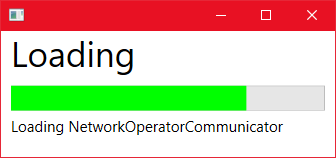
\includegraphics[width=8cm]{loading.png}
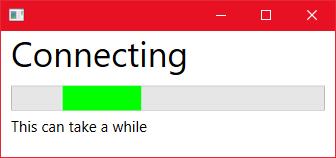
\includegraphics[width=8cm]{connecting.png}
\centering
\end{figure}
Po spuštění se zobrazí načítací obrazovka, která zobrazuje informace o průběhu načítání pluginů a procesu připojování k síti. Zprávy jsou do GUI předávány z jádra NetworkOperatoru, přijemž jejich odesílatel je jádro a příjemci jsou za tímto účelem rozšířené ovládací prvky (konkrétně dva TextBlocky a jeden ProgressBar). Po dokončení se zobrazí ovládací panel.

\subsubsection{Ovládací panel}
\begin{figure}[H]
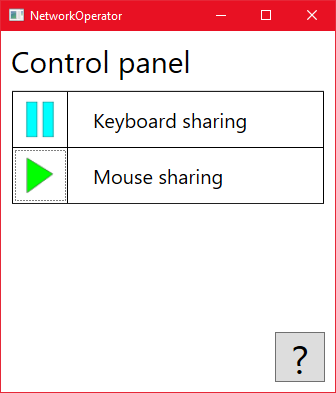
\includegraphics[width=8cm]{control-panel.png}
\centering
\end{figure}

Obsahuje tabulku všech dostupných operací, která má dva sloupce. V prvním sloupci je tlačítko pro změnu stavu operace obsahující ikonu reprezentující výsledný stav operace po provedení změny. Běžící operace jde pozastavovat a pozastavené operace spouštět.\\\\
Ve druhém sloupci je název operace. Pokud na něj uživatel klikne, zobrazí se přehled dané operace.\\\\
Tato tabulka je napsána jako listview, vzhled jehož položek je řízen datovou šablonou.\\\\
Dále zde je tlačítko s otazníkem, na které když uživatel klikne, otevře se dokumentace NetworkOperatoru ve výchozím webovém prohlížeči uživatele.

\subsubsection{Přehled běžící operace}
\begin{figure}[H]
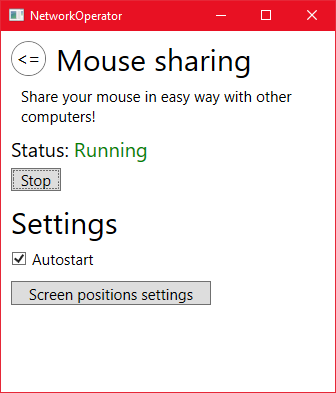
\includegraphics[width=8cm]{running-operation-overview.png}
\centering
\end{figure}

V přehledu lze nalézt název operace, krátký popis operace, ukazatel stavu operace, tlačítko umožňující změnu stavu operace a nastavení.\\\\
Součástí nastavení je vždy zaškrtávací box s nápisem "Autostart", kterým půjde upravovat, zdali se daná operace (její provádění) spustí po načtení NetworkOperatoru.\\\\
Dále může být součástí nastavení tlačítko s nějakým nápisem, na které když uživatel klikne, otevře se konfigurační okno dané operace. Toto tlačítko se zobrazí právě tehdy, když operace obsahuje ve své konfiguraci (vlastnost operace typu Configuration obsahující seznam objektů) instanci potomka třídy System.Windows.Window. Zobrazený nápis je vyčten ze stejné konfigurace.

\paragraph{Tlačítko zpět}
Vždy se nachází vedle nadpisu daného okna a vrací GUI o jeden krok zpět, na tu část GUI, ze které se na tu současnou uživatel dostal. Toto tlačítko se vždy chová stejně.

\subsubsection{Přehled zastavené operace}
\begin{figure}[H]
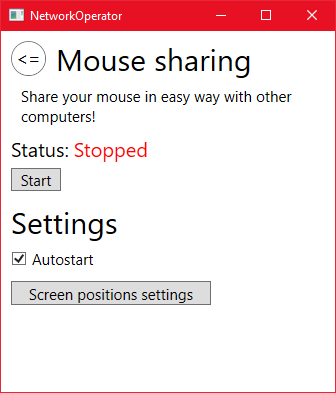
\includegraphics[width=8cm]{stopped-operation-overview.png}
\centering
\end{figure}

Po zastavení operace kliknutím na tlačítko "Stop" vypadá přehled operace jako na obrázku výše.

\subsubsection{Konfigurace vzájemného rozmístění počítačů}
\begin{figure}[H]
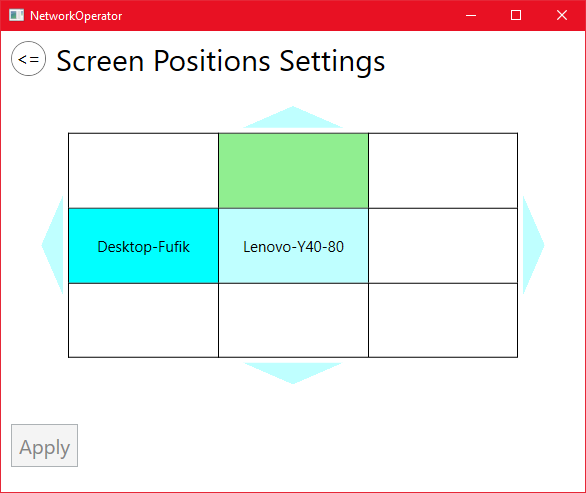
\includegraphics[width=12cm]{screen-positions-settings-green-field.png}
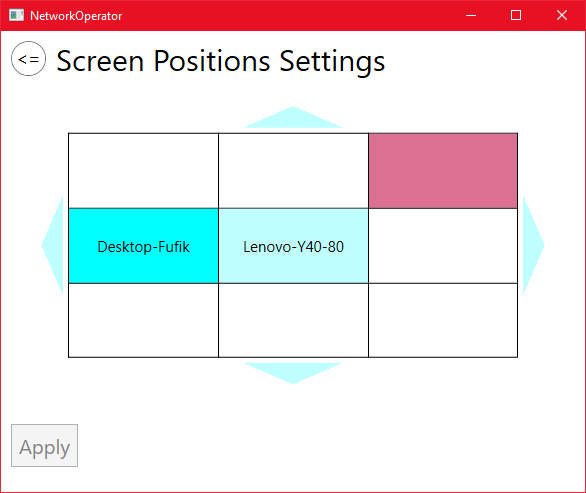
\includegraphics[width=12cm]{screen-positions-settings-red-field.png}
\centering
\end{figure}

Konfigurace vzájemného rozmístění počítačů funguje tak, že ve chvíli, kdy uživatel klikne na nějaké pole obsahující název počítače (řetězec), mohu tento počítač přesunout na nějaké jiné pole, říkejme mu cílové. Cílové pole vybírám kliknutím. Je-li na cílovém poli počítač, dojde k prohození vybraných počítačů, je-li pole prázdné a po najetí myší nad něj se obarví zeleně, dojde po kliknutí k přesunu počítače na cílové pole, pokud se obarví červeně, nelze na toto pole počítač přesunout (došlo by ke vzniku invalidní konfigurace). Z matice komunikantů, která je vyšší nebo širší než 3x3, je vždy viditelná podmatice o velikosti 3x3, která slouží jako náhled do vybrané části vetší matice. Pokud lze výběr v určitém směru posunout, rozsvítí se (jinak bledě modrá) šipka v daném směru. Po kliknutí na tlačítko "Apply" je nová konfigurace uvedena v platnost a v okamžik ukončení programu uložena na disk.

\subsection{Proces ukončení}
Ve chvíli, kdy uživatel ukončí program, zmizí GUI, zastaví se probíhající operace, NetworkCommunicator se odpojí od sítě a ukončí se všechna vlákna, čímž se ukončí i vlastní program. Uživatel by měl mít z ukončení NetworkOperatoru pocit, že je "hned" hotové.

\subsection{Cílová platforma}
Program je napsán v C\#u (a XAMLu), ale přímo používá Windows API, což způsobilo závislost programu na operačním systému Windows. Druhý důvod, proč je NetworkOperator kompatibilní pouze s Windows, je použití WPF k naprogramování GUI.\\\\
Testování bylo prováděno na počítači s Windows 7 a Windows 10, oboje aktualizované na současnou verzi, kompatibilita s jinými verzemi Windows zvláštním způsobem ověřována nebyla, ovšem program je napsán tak, aby pracoval na všech Microsoftem podporovaných desktopových verzích Windows.

\section{Splnění požadavků jednotlivých předmětů}
V následujícím seznamu je ke každému předmětu uvedeno, co za technologii probíranou na přednáškách k danému předmětu jsem netriviálně použil ve svém zápočtovém programu:
\begin{enumerate}[leftmargin=5mm]
\item NPRG035 (C\# - zima) - bez specifikace (pravděpodobně všechno)
\item NPRG038 (.NET I) - síťování, reflection, vláknování
\item NPRG057 (.NET II) - spolupráce C\#u a C++
\item NPRG064 (.NET UI) - WPF
\end{enumerate}

Celková velikost všech cs souborů vzniklých při psaní NetworkOperatoru dosahuje necelých 350kB, tudíž požadovaná minimální velikost 120kB při odevzdání po 8. 9. 2017 je splněna.

\end{document}
